\chapter{Erhebung der Anforderungen an das neue Korrelationsformat}\label{ch:anforderungen}


\section{Methode zu Erhebung der Anforderungen}

Zur Herleitung der Anforderungen an das neue Korrelationssystem wird zunächst die proprietäre Produktmodellierung der \metaeffektsp beschrieben, die in den meisten Fällen als Ausgangspunkt der Produktidentifikation dienen wird.
Aus diesem werden die unterschiedlichen relevanten Software-Ökosysteme vorgestellt und wie sich diese in den Software-Inventaren darstellt.
Anschließend wird der intern entwickelten Schwachstellenscanners vorgestellt, und das darin bisher verwendete Korrelationsformat zur Zuordnung von Komponenten mit ihren anderen Repräsentationen.
Das bestehende Format wird anschließend auf seine Schwächen und Herausforderungen untersucht, woraus die Anforderungen an das neue Korrelationsformat abgeleitet werden.


\section{Interne Produktmodellierung der \metaeffektlg}\label{sec:metaeffekt-inventory-format}

Wie alle Datentypen im Inventar basieren auch Artefakte auf Key-Value-Pairs, einer frei definierbaren Zuordnung von Textschlüsseln zu Textwerten.
Dieses Format wurde gewählt, um möglichst einfach Änderungen und neue Felder einführen zu können, ohne Schemata definieren und ändern zu müssen.
Komplexere Werte als flache Texte werden z.B.\ automatisch als JSON-Objekte serialisiert und beim Einlesen wieder als Objekte deserialisiert.

Für Artefakte ist die zugrunde liegende Struktur mit einigen Basis-Feldern für alle Software-Ökosysteme die gleiche, jedoch unterscheidet sich je nach Ökosystem die tatsächliche Verwendung der Felder.
Jedes Ökosystem hat somit eine übliche Menge an Feldern, mit denen eine Komponente beschrieben wird, die typischerweise ausgefüllt werden.

Beispielhafte Artefakte aus dem Java/Maven-Ökosystem sind in \autoref{tab:inventory-artifact-entries} dargestellt.

\begin{table}[ht]
    \caption{Beispielhafte Artefakteinträge in einem Software-Inventar}
    \label{tab:inventory-artifact-entries}
    \centering
    \begin{tabular}{llll}
        \toprule
        \textbf{Id}                  & \textbf{Component}         & \textbf{Group Id}        & \textbf{Version} \\
        \midrule
        commons-codec-1.15.jar       & Apache Commons Codec       & commons-codec            & 1.15             \\
        commons-collections4-4.1.jar & Apache Commons Collections & org.apache.commons       & 4.1              \\
        slf4j-api-1.7.36.jar         & SLF4J                      & org.slf4j                & 1.7.36           \\
        log4j-api-2.14.0.jar         & Apache Log4j               & org.apache.logging.log4j & 2.14.0           \\
        \bottomrule
    \end{tabular}
\end{table}

Da das Datenmodell tabellarisch angeordnet ist und damit in Tabelleneditoren mit mehreren Tabellenblättern abbildbar ist, wird es häufig in menschenlesbarer Form als \texttt{.xlsx} oder ähnlichen Formaten exportiert.

\subsection{Analyse bestehender Softwareinventare}

Da die Darstellungsweisen von Artefakten unterschiedlicher Software-Ökosysteme in den \metaeffekt-Software-Inventaren nicht vollständig normiert sind, wurde ein Datensatz mit den Artefakten aus 1820 realen Software-Inventaren von unterschiedlichen Quellen in einer Datenbank aggregiert und auf Muster untersucht.
Es stellt sich heraus, dass in den meisten Fällen die Art eines Artefakts durch eine Kombination von drei Attributen ableiten lässt: \texttt{Type}, \texttt{Component Source Type} und \texttt{Ecosystem}.
Nicht immer sind alle gesetzt, und manchmal kommt es auf die Kombination mehrerer an.

Das Attribut \texttt{Ecosystem} in Artefakten entspricht dem \texttt{type}-Attribut in \acrshortpl{purl} und kann von den erzeugenden Prozessen nur dann aufgefüllt werden, wenn auch eine \acrshort{purl} angegeben ist.
Fehlt dieses, kann meist \texttt{Component Source Type} für eine allgemeine Klassifikation und \texttt{Type} für die spezifischere Einordnung in ein zweistufiges hierarchisches Modell verwendet werden.
Leider wurden in dem Datensatz oft Artefakte komplett ohne Typ-Information gefunden, in diesen Fällen müssen weitere Algorithmen zur Erkennung etwa basierend auf Dateiendungen oder anderen Attributen entwickelt werden.

Ein Auszug aus den Werten des \texttt{Ecosystem}-Attributs:
\texttt{npm}, \texttt{gem}, \texttt{github}, \texttt{cpan}, \texttt{wut}, \texttt{docker}, \texttt{internal}, \texttt{conan}, \texttt{deb}, \texttt{nuget}, \texttt{generic}, \texttt{maven}, \texttt{rpm}, \texttt{pypi}, \texttt{golang}, \texttt{apk}.

Die beobachteten Werte aus den Attributen \texttt{Component Source Type} und \texttt{Type} reichen von Ökosystemen und Dateitypen bis hin zu Begriffen aus der Betriebssystem- und Gerätetreiberdomäne.
Da sich einige Typen in unterschiedlichen Schreibweisen oder Bedeutungen wiederholen, kann von einer stark heterogenen Entstehung der Artefakte ausgegangen werden.
Die folgenden Kombinationen aus \texttt{Component Source Type} und \texttt{Type} konnten im Datensatz gefunden werden:

\begin{itemize}
    \itemsep0em
    \item \texttt{generic-version → package}
    \item \texttt{java-runtime → package}
    \item \texttt{pwa-module → web-module}
    \item \texttt{bower-module → web-module}
    \item \texttt{npm-module → nodejs-module, web-module}
    \item \texttt{jar-module → module}

    \item \texttt{<empty> → (hardware/drivers) storage controller, imaging hardware, operating-system, audio hardware, power driver, mouse, Universal Serial Bus controller driver, data storage, multimedia output device, device connector, firmware driver, storage driver, printer driver, power supply, extension module, disk drives driver, printer, input device, audio driver, computer driver, display driver, processing core, driver, sensor, multimedia driver, appliance, security token, sound hardware, network driver, mouse driver, usb controller driver, security device driver, Bluetooth driver, keyboard, controller, operating system, display, imaging driver, port driver, security hardware, input device driver, system device driver, keyboard driver, print queue driver, processor driver, software device driver, networking hardware, board}
    \item \texttt{<empty> → (other) package, python-module, nodejs-module, bios, file}
    \item \texttt{<empty> → <empty>}
\end{itemize}

Bei einer Sichtung des Quellcodes einiger Entstehungsquellen von Artefakten konnte die große Auflistung der Hardware- und Betriebssystemtypen in dem Windows-Inventar-Extraktor System gefunden werden, die restlichen sind über diverse Extraktoren verteilt oder werden extern aufgefüllt und damit nicht einheitlich nachvollziehbar.

% erkennungsrichtlinien für einzelne ökosysteme


\section{Analyse des Schwachstellenscanners der \metaeffektlg}

% “The results show that the method describe” (Sanguino and Uetz, 2017, p. 22) Sanguino_Uetz_2017
%   auf diese art und weise die shortcomings unseres scanners beschreiben
% vor allem problematisch wenn es keine CPE gibt weil dann oft doch eine gefunden wird
% subsection über effective CPE

\subsection{Effective CPE Calculation}\label{subsec:effective-cpe-calculation}


\section{Aktuelles Korrelationsformat zur Modifikation von Artefaktmetadaten}\label{sec:current-correlation-format}

Das Korrelationsformat wurde 2021 entwickelt, um manuelle Nachkorrekturen an den durch die \enquote{CPE Derivation} automatisch abgeleiteten \acrshort{cpe}-Identifikatoren zu ermöglichen.
Während der Hauptanwendungsfall daraus besteht, fehlerhafte oder unpassende \acrshort{cpe}-Zuordnungen zu korrigieren, ermöglicht es die Modifikation beliebiger Artefaktattribute, und wurde so über die Zeit für viele weitere Anwendungsfälle eingesetzt.

Das Format basiert auf \acrfull{yaml} und folgt einem zweistufigen Modell:
Über einen Selektor werden Regeln für die Auswahl von Artefakten definiert, und dann eine Reihe an Modifikationen, die an diesem Artefakt vorgenommen werden sollen.
Jeder Korrelationseintrag kann aus den folgenden Attributen bestehen, wobei mindestens ein \texttt{affects} und eine Modifikationsoperation definiert sein muss.
Ein kleines Beispiel bei dem eine \acrshort{cpe} zu einem Artefakt hinzugefügt wird kann in \autoref{lst:correlation-initial-example} gefunden werden, ausführlichere Beispiele mit Beschreibungen werden nach der Formatbeschreibung aufgeführt.

\begin{lstlisting}[style=yaml,caption={Korrelationseintrag für die Java-Komponente Liquibase},label={lst:correlation-initial-example}]
- affects:
    - Id: liquibase-*.jar
    - Id: org.liquibase.liquibase-*.jar
  append:
    Additional CPE URIs: cpe:/a:liquibase:liquibase
\end{lstlisting}

\paragraph{Artefakt-Selektion}
Die \texttt{affects}-Sektion eines Eintrages muss immer vorhanden sein und legt fest, auf welche Artefakte sich der Eintrag beziehen soll.
Dabei wird in einer Listenstruktur eine Menge an Attribut-Wert-Paaren angegeben, die auf der Ebene der Liste logisch als ODER-Verknüpfung interpretiert werden und die Attribute innerhalb der Liste mit einer UND-Verknüpfung verbunden sind.
Das bedeutet, dass bereits ein zutreffendes Listenelement ausreicht, um einen Treffer zu erzielen, aber innerhalb jedes Elements müssen alle angegebenen Attribut-Werte-Paare auf das zu prüfende Artefakt zutreffen.
Die betroffenen Attribute können beliebige Felder aus einem Artefakt sein (etwa \texttt{Id}, \texttt{Component}, \texttt{Group Id}, \texttt{Type}, \ldots).
Es ist dadurch möglich domänenübergreifende Selektionskriterien zu formulieren.

Optional kann ein \texttt{ignores}-Block definiert werden, der vom Aufbau her der \texttt{affects}-Sektion entspricht, aber die Logik umkehrt.
Sobald einer der Listeneinträge mit einem Artefakt erfolgreich verglichen wurde, wird das Artefakt von dem Eintrag ausgeschlossen.
Damit können Ausnahmen und Abgrenzungen zu ähnlichen Artefakten erstellt werden, etwa bei Artefakten mit ähnlichen Namen aber unterschiedlichen Ökosystemen.

Die zu vergleichenden Werte der Attribut-Wert-Paare unterstützen mehrere Matching-Modi.
Im einfachsten Fall wird ein Text auf Gleichheit mit dem Attributinhalt verglichen, hierzu wird der Text einfach aufgeführt.
In diesem einfachen Vergleichsmodus können Platzhalterzeichen verwendet werden, so steht ein Sternchen (\texttt{*}) für beliebig viele Zeichen und ein Fragezeichen (\texttt{?}) für ein einzelnes beliebiges Zeichen.
Über zwei Stufen können sich die Werte regulären Ausdrücken annähern:
Ähnlich zu der Notation wie sie in JavaScript verwendet wird \autocite{MdnRegularExpressions2025} können durch das Anhängen von einem Schrägstrich und einer Menge an Flags wie in \enquote{\texttt{/i}} beispielsweise auch case-insensitive Vergleiche durchführen, ohne vollständig auf reguläre Ausdrücke zu wechseln.
Die vollständige Nutzung von regulären Ausdrücken wird ermöglicht, wenn das Muster von vorne und hinten durch \enquote{\texttt{/}} eingerahmt wird.
Durch diese inkrementelle Syntax kann einfach zwischen unterschiedlichen Matching-Modi gewählt werden.

\paragraph{Artefakt-Modifikation}
Sobald ein Artefakt durch einen Eintrag als betroffen erkannt wird, werden die im zweiten Teil des \acrshort{yaml}-Blocks definierten Modifikationen angewandt.
Auch hier gibt es unterschiedliche Weisen, die Attribute der Artefakte zu modifizieren, wobei sich das allgemeine Schema bei den meisten gleicht:
Jede Art an Modifikation führt eine Menge an Attributen, die jeweils einen Text-Wert zugeordnet haben.
Die am häufigsten verwendete Operation ist \texttt{append}, die auf \acrfull{csv}-Attributen angewendet wird, und den angegeben Wert entweder mit einem Komma getrennt an den vorhandenen angehängt wird, oder direkt gesetzt wenn noch keiner vorhanden ist.
Typischerweise betrifft dies \acrshortpl{cpe}, die nachträglich als gültig oder unpassend erkannt wurden und zu einer entsprechenden Liste hinzugefügt werden sollen.
Ähnlich operiert \texttt{remove}, womit auch hier der auf dem Artefakt vorhandene Wert und der im Korrelationseintrag angegebene Wert als \acrshort{csv}-Werte interpretiert und an Kommas getrennt werden und die Schnittmenge der beiden Listen vom Artefakt-Attribut entfernt werden.
\enquote{overwrite} ersetzt den kompletten Inhalt eines Attributs mit einem neuen Werte und \enquote{clear} entfernt ein Attribut von einem Artefakt.

\bigskip

Mit diesen Methoden, auf Artefakte zuzugreifen, können potenziell alle Transformationen an Artefakten durchgeführt werden, die von Interesse sind.
Im Kontext der \acrshort{cpe}-Zuordnung sind besonders die drei Felder relevant, die auch schon in \autoref{subsec:effective-cpe-calculation} aufgeführt wurden:
\texttt{Additional CPE URIs}, \texttt{Inapplicable CPE URIs} und \texttt{CPE URIs}.

Ein Konsens, der sich über die Zeit aus Gründen der Nachvollziehbarkeit geformt hat, ist das Hinzufügen eines Kommentarblocks vor dem Korrelationseintrag mit Informationen über das Artefakt, für den der Eintrag angelegt wurde und eine Begründung, warum er nötig ist.
Dieser Kommentar kann beliebige Begründungen enthalten, etwa Verweise auf Dokumentationen, URLs zu Projektseiten oder kurze Erklärungen, warum etwa eine bestimmte \acrshort{cpe} als passend oder unpassend eingestuft wurde.
Bei späteren Revisionen und Diskussionen im Team erleichtert das die Nachvollziehbarkeit vergangener Entscheidungen.

\subsection{Beispiele zu Korrelationsdaten}

\paragraph{Beispiel 1: snappy-1.1.8}
In \autoref{lst:correlation-snappy} ist ein Beispiel aufgeführt, bei dem ein Artefakt \texttt{snappy-1.1.8} als ein Linux Package (Typ \texttt{package}) in einem Softwareinventar identifiziert wurde.
Der CPE URI Derivation-Algorithmus hat in das Attribut \texttt{Derived CPE URIs} seine Identifikation aufgenommen, nämlich \texttt{cpe:/a:knplabs:snappy}.
Vom Namen her sieht diese Identifikation vielleicht überzeugend aus, allerdings stellt sich dies als eine Fehlidentifikation heraus, denn die \acrshort{cpe} verlinkt in ihren Metadaten auf \url{https://github.com/KnpLabs/snappy}, was eine PHP Bibliothek ist und kein Linux Paket.
Erst bei einer manuellen Suche kommt eine zweite \acrshort{cpe} hervor, \texttt{cpe:/a:google:snappy}, die tatsächlich ein Linux Paket darstellt welches nicht nur vom Namen her passt, sondern auch von der Versionsreichweite der veröffentlichten Versionen.
Allerdings wurde auch eine Java-Bibliothek mit demselben Namen identifiziert, also mussten die entsprechenden jar-Dateien über \texttt{ignores} ausgeschlossen werden.
Alternativ hätte auch das \texttt{affects} mit \texttt{Type: package} erweitert werden können, um die Artefakte so zu limitieren.
So ergibt sich der gesamte Eintrag, in dem allgemein alle mit \texttt{snappy-} startenden Artefakte ausgewählt werden, die mit \texttt{.jar} hinten exkludiert und auf den Restlichen die jeweiligen \acrshortpl{cpe} als anwendbar oder nicht in die Artefakt-Attribute mit aufgenommen werden.
In der Praxis würde nun noch ein weiterer Eintrag für die PHP-Bibliothek angelegt werden, der auf den korrekten \texttt{Type} prüft.

\begin{lstlisting}[style=yaml,caption={Korrelationseintrag für Snappy-Komponenten},label={lst:correlation-snappy}]
# Id: snappy-1.1.8
# Component: snappy
# Version: 1.1.8
# Type: package
# Derived CPE URIs: cpe:/a:knplabs:snappy
# reason:
#   cpe:/a:knplabs:snappy --> https://github.com/KnpLabs/snappy --> "PHP library allowing thumbnail, snapshot or PDF generation from a url or a html page." --> PHP library
#   cpe:/a:google:snappy --> https://github.com/google/snappy --> https://pkgs.alpinelinux.org/package/edge/main/x86/snappy --> linux package --> matches this package version range
#   ignore https://mvnrepository.com/artifact/org.xerial.snappy/snappy-java
- affects:
    - Id: snappy-*
  ignores:
    - Id: snappy-*.jar
  append:
    Inapplicable CPE URIs: cpe:/a:knplabs:snappy
    Additional CPE URIs: cpe:/a:google:snappy
\end{lstlisting}

\paragraph{Beispiel 2: Microsoft Windows 10 (Version 21H2)}

Auch nicht-\acrshort{cpe}-Attribute können auf Artefakten ergänzt werden.
In dem Beispiel in \autoref{lst:correlation-win-10-21H2} wird eine Microsoft-Produkt-Id zu dem Betriebssystem Windows 10 in der Version 21H2 zugeordnet.
Der \href{https://github.com/org-metaeffekt/metaeffekt-documentation/blob/bd184b2889d5421b5a71dcd26c1ac0ffc63d07e7/metaeffekt-vulnerability-management/data-mirror/msrc/understanding-data.md}{Dokumentationeintrag zu den Microsoft-Datenquellen} und in \autoref{subsec:msrc-product-ids} wird das Microsoft-Produktidentifikator-Ökosystem näher erklärt, aber prinzipiell haben alle versionierten Produkte in der Microsoft-Datenbank eine eindeutige numerische Id, unter der Schwachstellen registriert werden.
Daher muss nur auf die exakten Attribute geprüft werden und dann kann die korrekte Produkt-Id zu dem Artefakt hinzugefügt werden.
Zusätzlich wird für das EOL-Ökosystem die entsprechende Produkt-Id \texttt{windows} hinzugefügt und eine für die Abfrage spezifische Version die in diesem Ökosystem verwendet werden muss.

\begin{lstlisting}[style=yaml,caption={Korrelationseintrag für Snappy-Komponenten},label={lst:correlation-win-10-21H2}]
# reason: https://learn.microsoft.com/de-de/windows/release-health/release-information
#   11931 --> Version 21H2 (OS build 19044) / Windows 10 Version 21H2 for x64-based Systems
- affects:
    - Id: Microsoft Windows 10*
      Version: 10.0.19044*
      Type: operating system
      Architecture: "*64*"
    - Id: Windows 10*
      Version: 10.0.19044*
      Type: operating system
      Architecture: "*64*"
  append:
    MS Product ID: "11931"
    EOL Id: windows
    EOL Overwrite Cycle Query Version: 10 21H2 (E)
\end{lstlisting}

\subsection{Correlation Utilities als Tool zur Korrelationsarbeit}

Da der Prozess ein gesamtes Software-Inventar durchzuarbeiten ohne weitere unterstützung von Tools recht aufwendig ist, wurden die \enquote{Correlation Utilities} entwickelt um den Prozess zu unterstützen.
Als eine Spring Boot Anwendung im Backend mit einem modularen und anpassbaren kachelbasierten Frontend kann hier ein Inventar in eine Tabellarische Form geladen und die Artefakte nach und nach durchgearbeitet werden.
In \autoref{fig:correlation-utilities-demo} kann die entsprechende Nutzeroberfläche gesehen werden.
Diese besteht links oben aus der Tabelle der Artefakte, mit farbigen Status-Indikatoren pro Zeile um schnell nach relevanten Metriken filtern zu können und einer Detailsicht mit allen Attributen des ausgewählten Artefakts unten.
Hier werden zudem über Web-Requests und lokale Datenbankabfragen im Backend diverse weitere nützliche Informationen und Links aggregiert und Internetsuchen vorbereitet, damit diese nicht über repetitive manuelle Suchen selbst durchgeführt werden müssen.

\begin{figure}
    \centering
    \makebox[\linewidth]{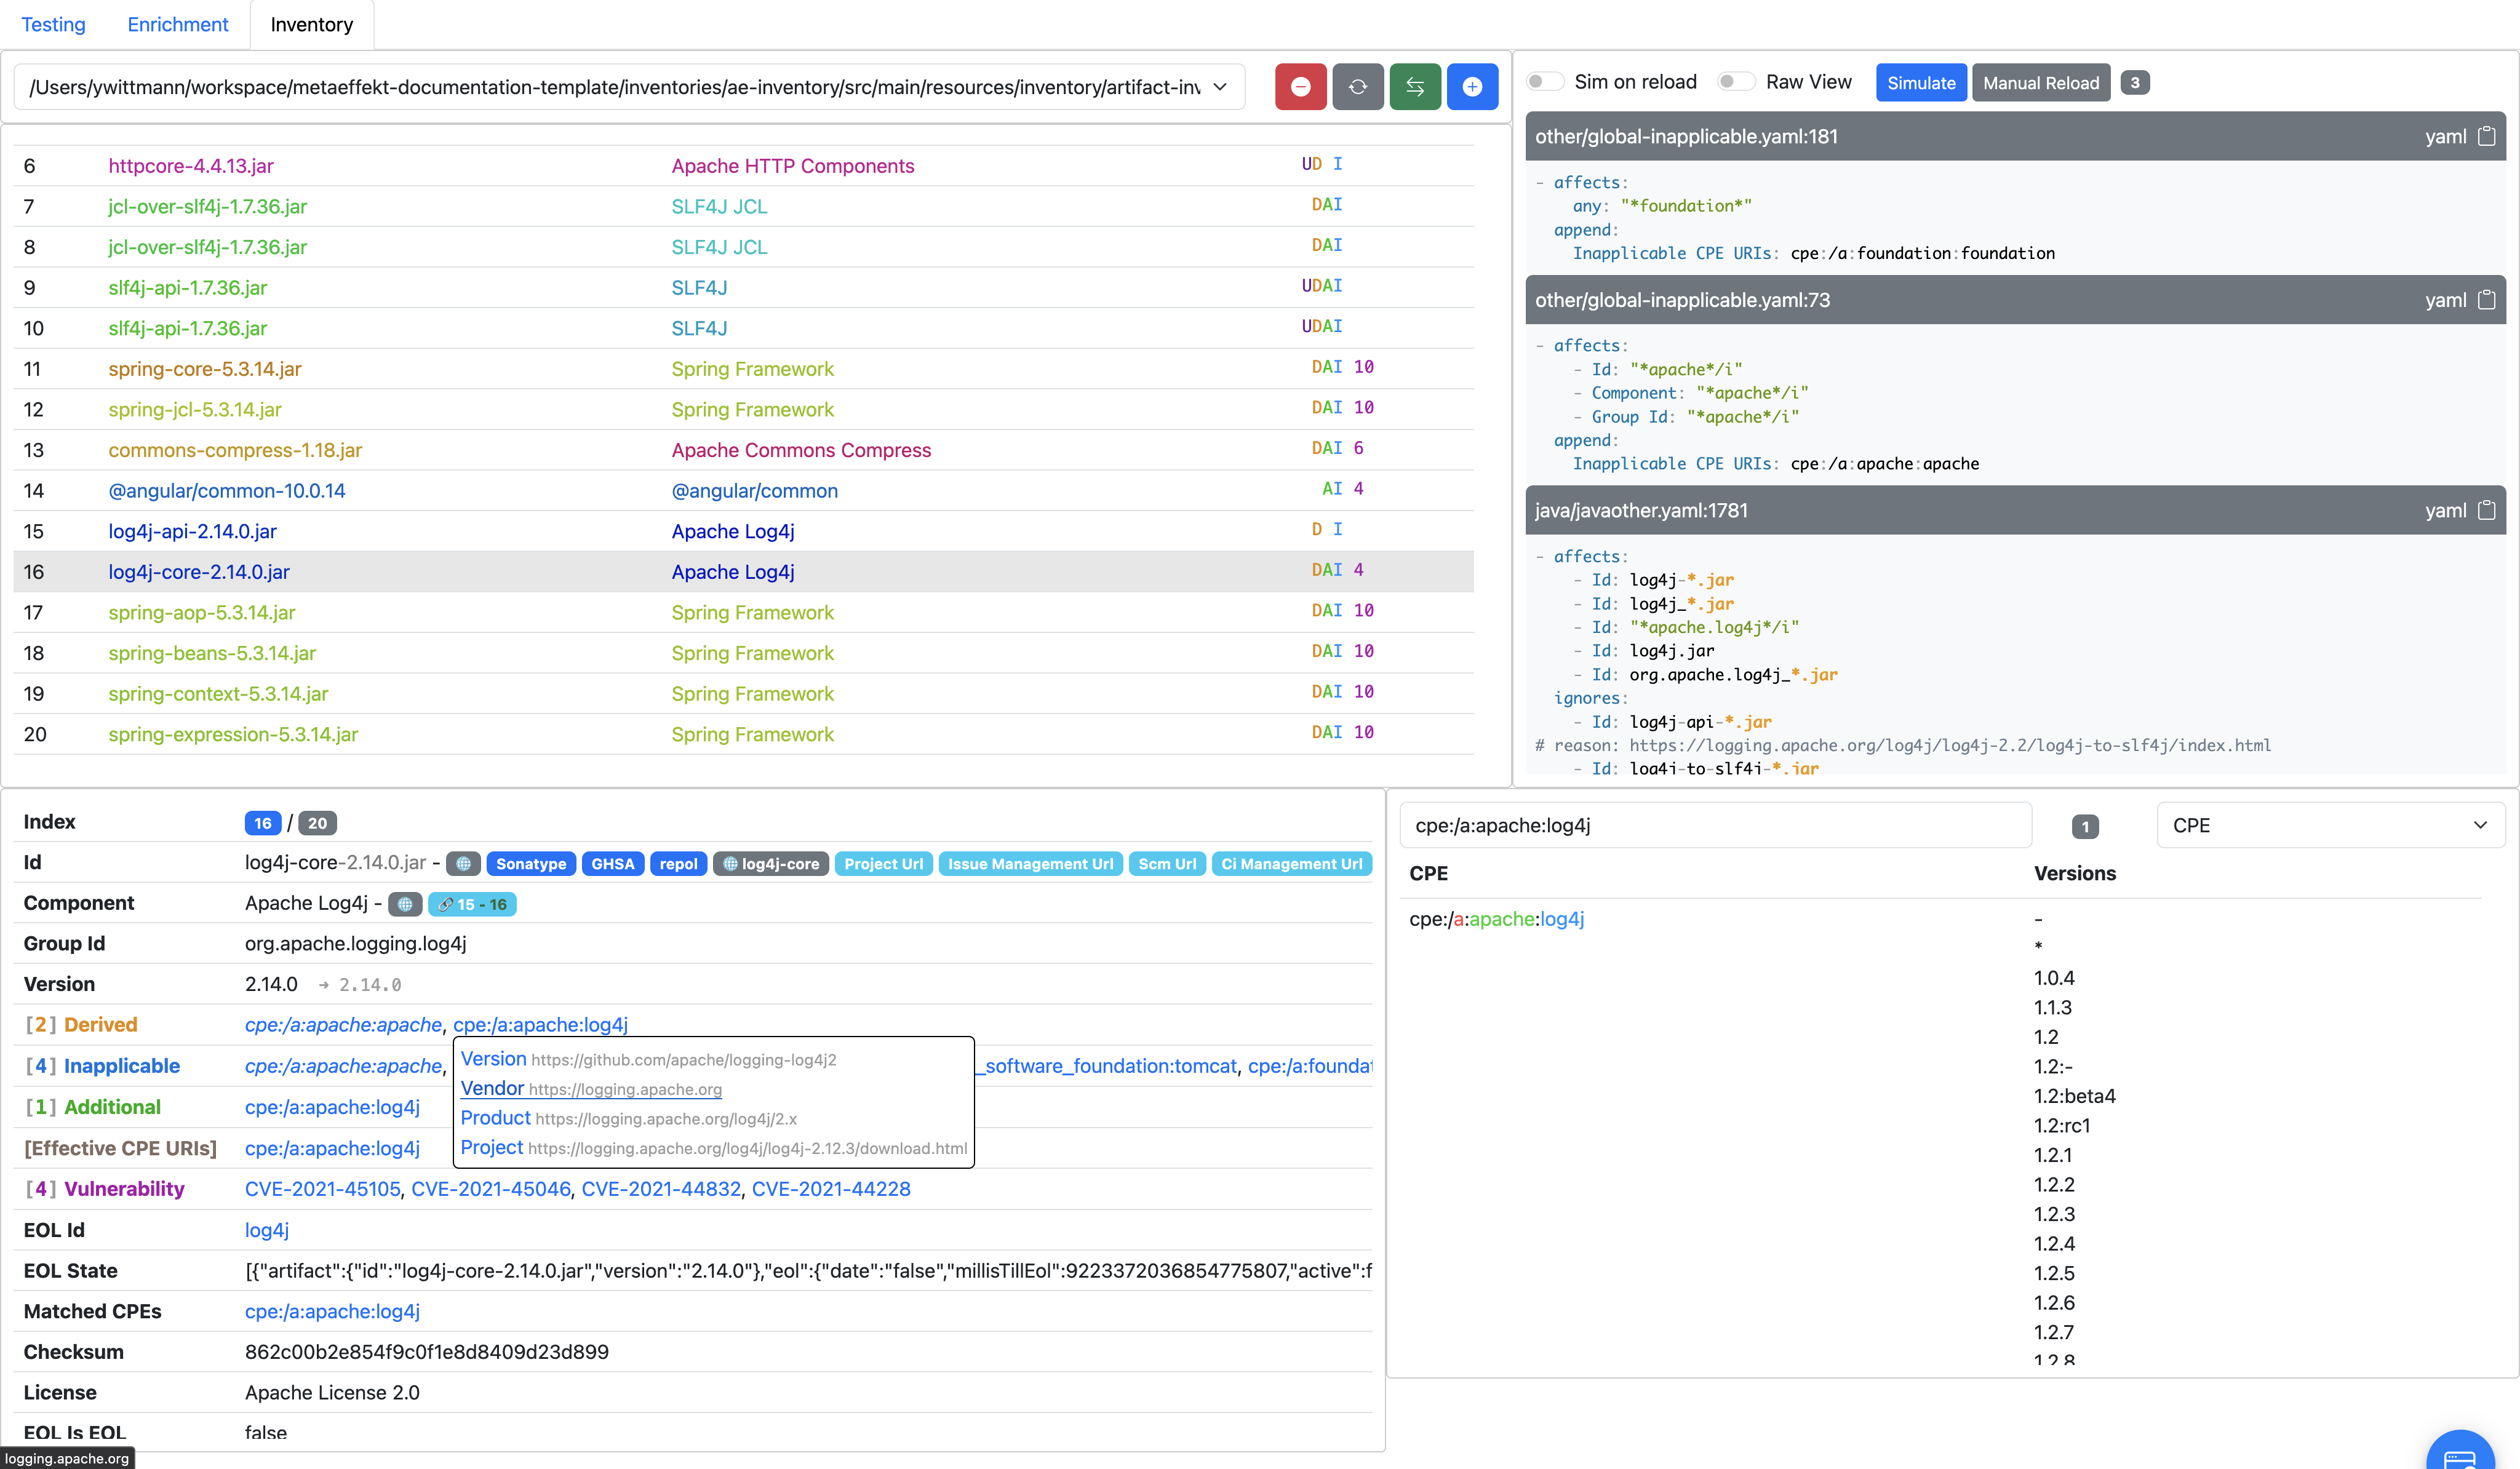
\includegraphics[keepaspectratio,width=1.3\linewidth]{../../images/correlation-utilities-demo}}
    \caption{Das Artefakt \texttt{log4j-core-2.14.0.jar} in den Correlation Utilities}
    \label{fig:correlation-utilities-demo}
\end{figure}

Auf der rechten Seite sind oben die vorhandenen Korrelationsdaten zu sehen, die auf das aktuelle Artefakt zutreffen und über eine Integration mit IntelliJ IDEA können über einen Klick die Einträge automatisch in der \acrfull{ide} geöffnet werden.
Zudem wird aufgrund von einigen bekannten Mustern ein neuer Korrelationseintrag mit Referenzen auf reale Daten vorgeschlagen, der mit einem Klick kopiert werden kann.
Die Daten werden automatisch bei Änderungen in den Dateien neu geladen und ausgewertet.

Unten rechts ist eine Datenbankabfragesicht, in der dedizierte Abfragen auf die lokalen Daten gemacht werden können, wie etwa \acrshort{cpe}-Versionen oder Referenzen zu finden oder nach Schwachstellen oder anderen Repräsentationen zu suchen.

% TODO: actually perform test, ask Julian
% \smallskip
% Nach einem internen Test hat sich herausgestellt, dass Mitarbeiter mit den Utilities mehr als 2.5-mal so schnell die selbe Arbeit in höherer Ergebnisqualität durchführen konnten, wie wenn sie dieses Tool nicht verwendet hätten.


\section{Schwächen und Herausforderungen des aktuellen Korrelationsformats}


\section{Auflistung der Anforderungen}

% “4.3. Data Types in Falcon” ([Cheramangalath et al., 2016, p. 6](zotero://select/library/items/4DG8G9J3)) ([pdf](zotero://open-pdf/library/items/QNYKYEH4?page=6&annotation=C7MKFAUG))
